\subsection{UC31 - Modifica menu' del ristorante}\label{usecase:31}
\begin{figure}[H]
    \centering
    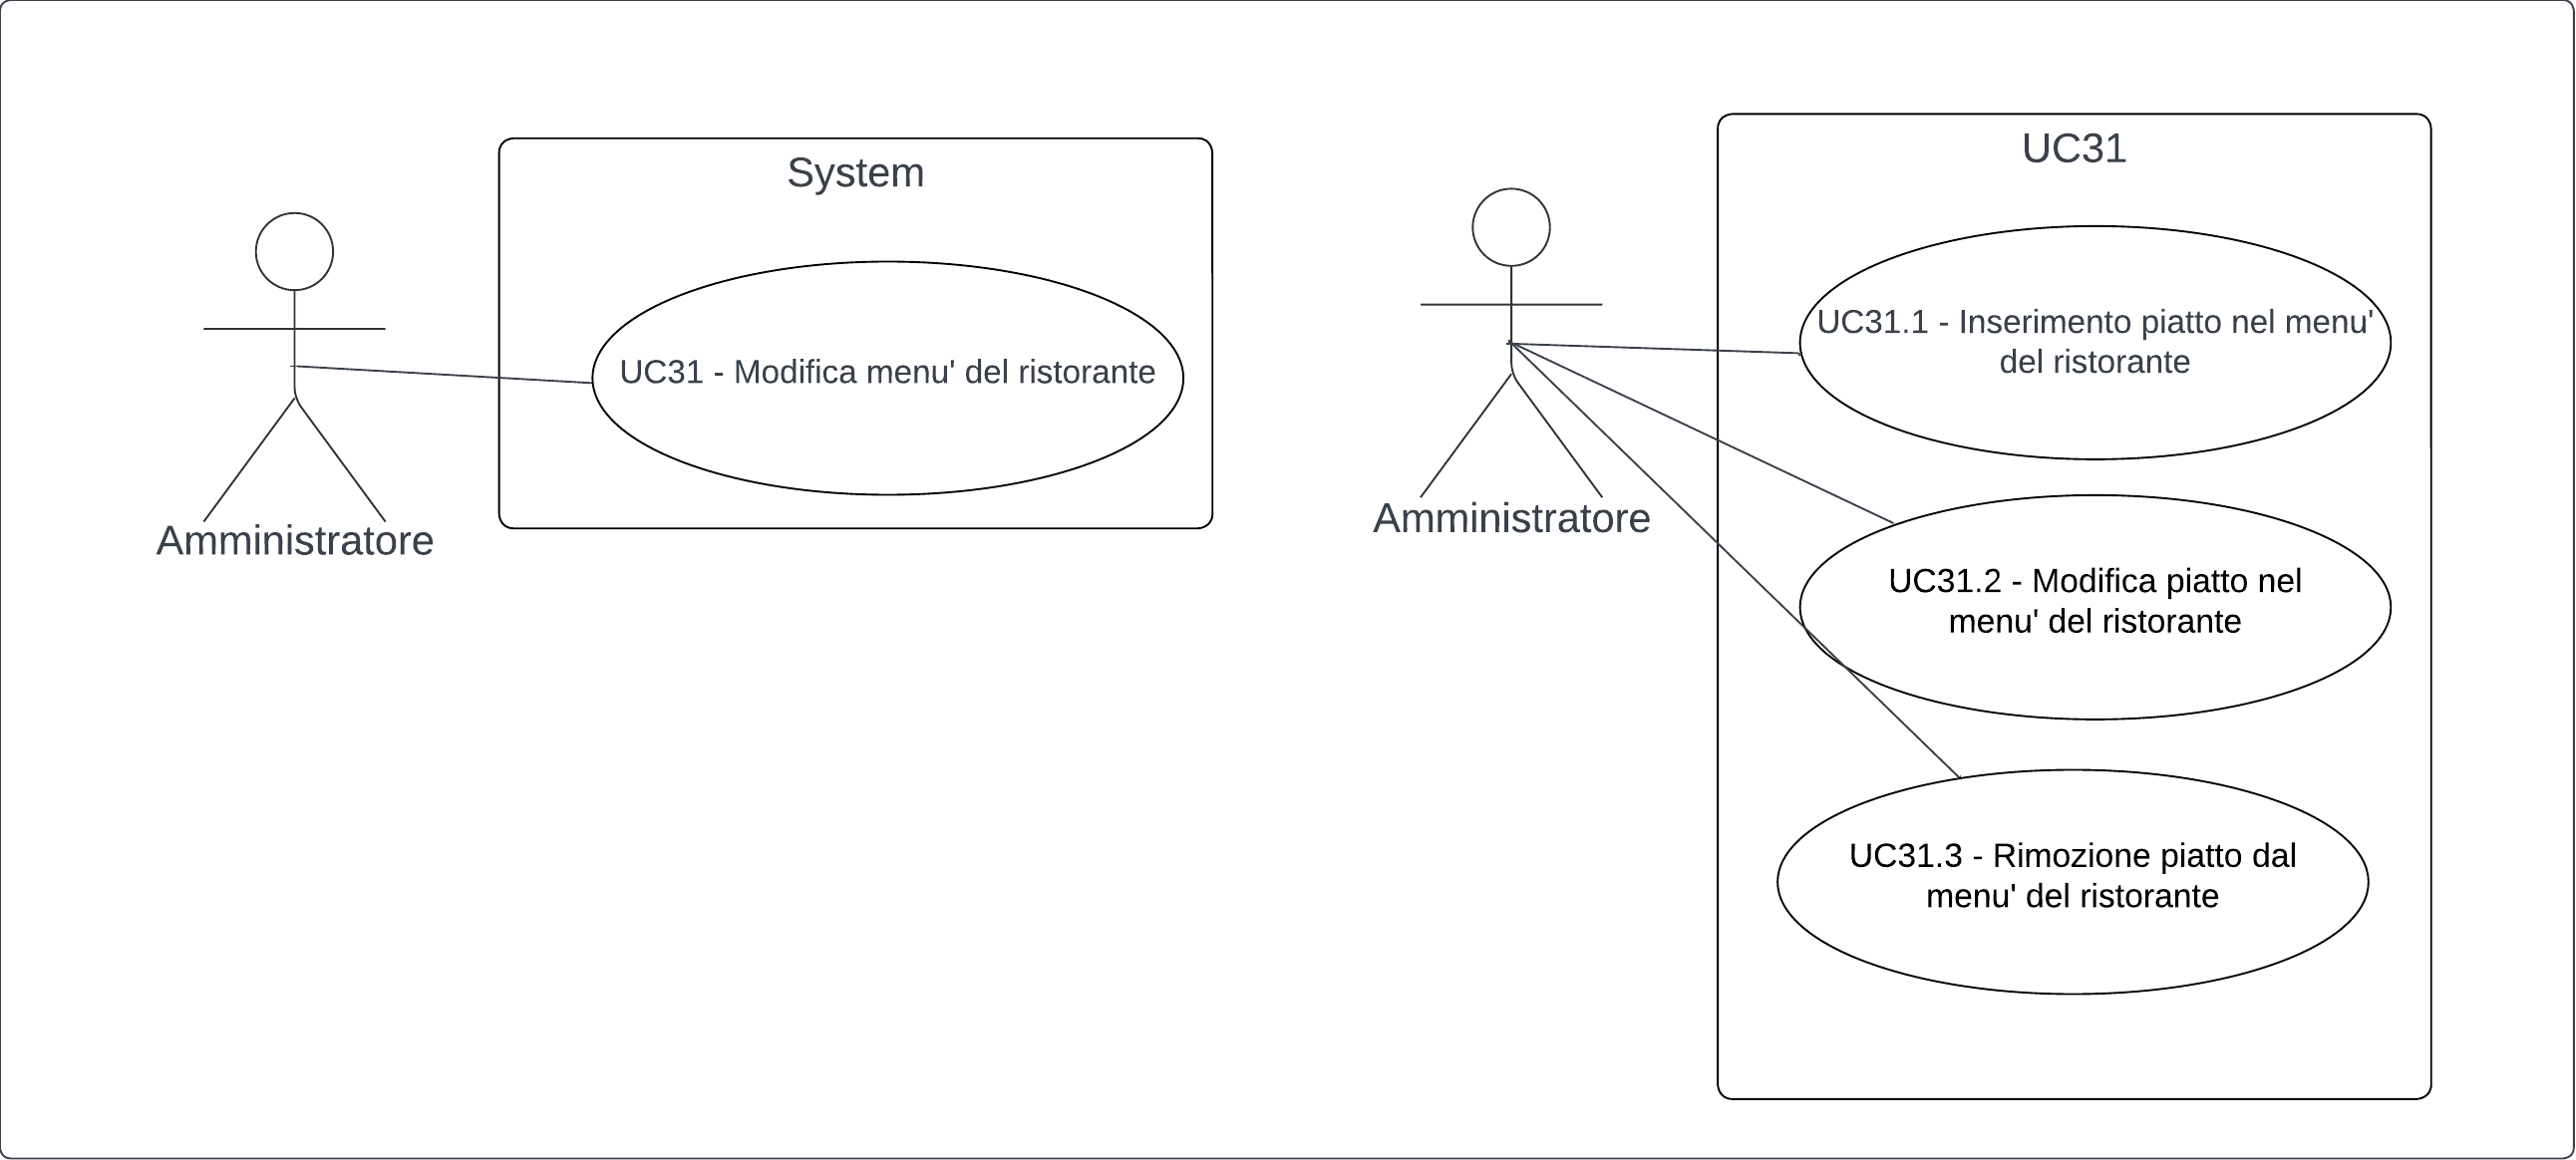
\includegraphics[width=0.9\linewidth]{ucd/UCD31.png}
    \caption{Modifica menu' del ristorante}
\end{figure}
\textbf{Attori}:
\begin{itemize}
    \item Amministratore.
\end{itemize}
\textbf{Precondizioni}:
\begin{itemize}
    \item L'utente è connesso al $\textit{sistema}_G$.
\end{itemize}
\textbf{Postcondizioni}:
\begin{itemize}
    \item L'utente ha modificato il menu' del proprio ristorante.
\end{itemize}
\textbf{Scenario principale}:
\begin{enumerate}
    \item L'utente può compiere le seguenti azioni per gestire il menu' del ristorante che gestisce:
    \begin{enumerate}
        \item Inserire un piatto nel menu' (\nameref{usecase:31_1});
        \item Modificare un piatto nel menu' (\nameref{usecase:31_2});
        \item Rimuovere un piatto dal menu' (\nameref{usecase:31_3});
    \end{enumerate}
    \item L'utente conferma le modifiche e il $\textit{sistema}_G$ le aggiorna.
\end{enumerate}